\serie{Calculer l'aire d'un parallélogramme}



\begin{exercice}[Avec un quadrillage]
Sachant que l'unité d'aire est le carreau, détermine l'aire de chaque figure suivante en utilisant des aires de parallélogrammes.
\begin{center}
    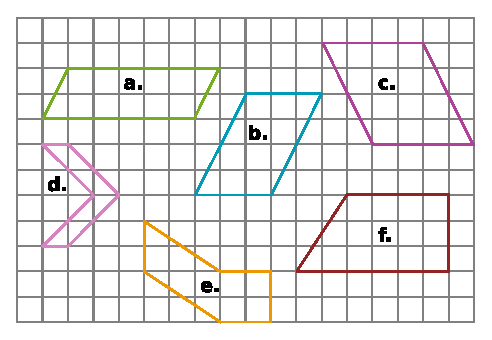
\includegraphics[width=\linewidth]{eeCD01}
\end{center}
\end{exercice}



\begin{exercice}[]
Calcule l'aire de chaque parallélogramme dont les dimensions sont données ci-dessous.
\begin{colenumerate}{1} 
\item Un côté mesure 6\,cm et la hauteur relative à ce côté mesure 4\,cm.
\item Un côté mesure 4,7\,dm et la hauteur relative à ce côté mesure 7,2\,cm.
\item Un côté mesure 2\,m et la hauteur relative à ce côté mesure 6,4\,cm.
\end{colenumerate} 
\end{exercice}

\begin{exercice}[]
Calcule la longueur demandée.
\begin{colenumerate}{1} 
\item L'aire du parallélogramme est 36\,cm\up{2} et l'un de ses côtés mesure 6\,cm. Combien mesure la hauteur relative à ce côté ?
\item L'aire du parallélogramme est 15,12\,cm\up{2} et l'une de ses hauteurs mesure 3,6\,cm. Combien mesure le côté associé à cette hauteur ?
\end{colenumerate} 
 
\end{exercice}

\begin{exercice}[Ne pas confondre !]
Calcule l'aire et le périmètre de ce parallélogramme tracé à main levée.
\begin{center}
    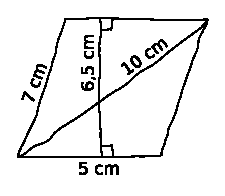
\includegraphics[width=.5\linewidth]{eeCD02}
\end{center}

\end{exercice}

\begin{exercice}[L'un dans l'autre]
Sur la figure suivante, les points $V$, $E$, $L$ et $U$ sont les milieux des côtés d'un rectangle $RATO$.

\begin{colenumerate}{1} 
\item Calcule l'aire de $RATO$, sachant que $RA =$8\,cm et $AT =$6\,cm.
\item Calcule l'aire de $VELU$ de deux façons.
\end{colenumerate} 

\begin{center}
    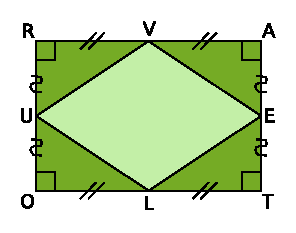
\includegraphics[width=.65\linewidth]{eeCD03}
\end{center}
 
\end{exercice}



\serie{Calculer l'aire d'un triangle}






\begin{exercice}[Avec un quadrillage (bis)]
Sachant que l'unité d'aire est le carreau, détermine l'aire des figures suivantes en utilisant des aires de triangles.

\begin{center}
    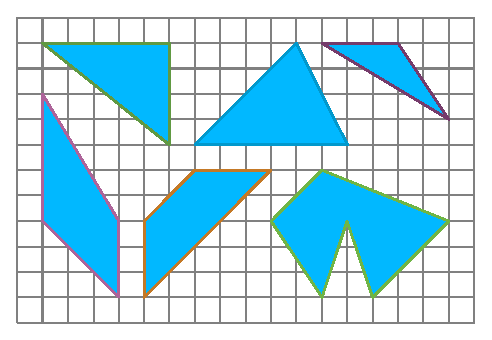
\includegraphics[width=\linewidth]{eeCD04}
\end{center}

\end{exercice}

\begin{exercice}[Calculer (mentalement !) pour construire]

\begin{colenumerate}{1} 
\item Trace un triangle $OIL$ rectangle en $O$ d'aire 15\,cm\up{2}.
\item Trace un triangle isocèle $EAU$ d'aire 12\,cm\up{2}.
\end{colenumerate} 
\end{exercice}



\begin{exercice}[]
En utilisant les données de l'énoncé, calcule l'aire du triangle $DEF$ puis déduis-en les longueurs $DK$ et $DF$.

\ImageDroite{$DE = 8$\,cm

	$EF = 5$\,cm
	
	$IF = 2,1$\,cm
	
	$EJ = 4,2$\,cm
	}{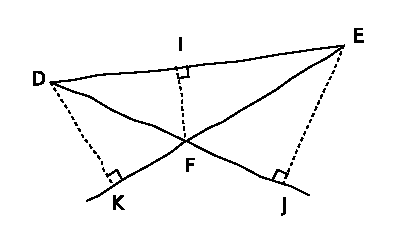
\includegraphics[width=.6\linewidth]{eeCD05}}
\end{exercice}



\serie{Cercles}



\begin{exercice}[Comparaison]

\begin{colenumerate}{1} 
\item Compare le périmètre de ces quatre figures. 

\begin{center}
    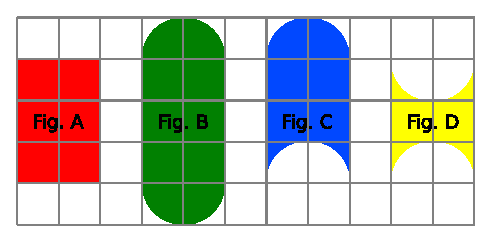
\includegraphics[width=\linewidth]{eeCD06b}
\end{center}
\item Compare l'aire de ces quatre figures. Justifie.
\end{colenumerate} 
\end{exercice}


\begin{exercice}[]
Calcule le périmètre des cercles suivants. Tu donneras la valeur exacte puis une valeur approchée au centième près.  

\begin{center}
    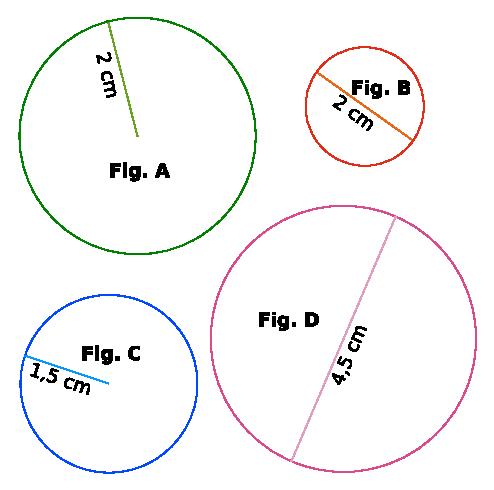
\includegraphics[width=\linewidth]{eeCD07}
\end{center}
\end{exercice}


\begin{exercice}[Trio de figures]

\begin{colenumerate}{1} 
\item Vincent affirme que les trois figures ci-dessous ont le même périmètre. A-t-il raison ?
 
\begin{center}
    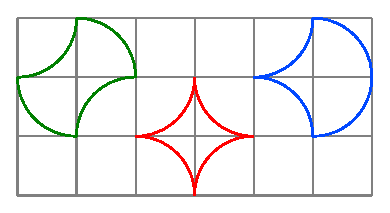
\includegraphics[width=.85\linewidth]{eeCD08}
\end{center}

\item Chaque carré a pour côté 1\,cm. Calcule le périmètre de ces trois figures.
\end{colenumerate} 
 
\end{exercice}

\begin{exercice}[]
Calcule le périmètre des cercles suivants. Tu donneras la valeur exacte puis une valeur approchée au dixième.

\begin{colenumerate}{2} 
\item Rayon : 3\,cm 
\item Rayon : 4,5\,cm
\item Rayon : 5\,dm
\item Diamètre : 7\,cm
\item Diamètre : 8\,cm
\item Diamètre : 25\,mm
\end{colenumerate} 
\end{exercice}

\begin{exercice}[]
On considère que l'équateur est un cercle de rayon 6 400\,km. Calcule le périmètre de l'équateur. Donne une valeur approchée au millier de kilomètres près.
\end{exercice}

\begin{exercice}[]
Calcule le périmètre de l'intérieur du stade Gerland de Lyon (il est constitué d'un rectangle et de deux demi-cercles). Tu donneras la valeur exacte et une valeur approchée au centimètre.

\begin{center}
    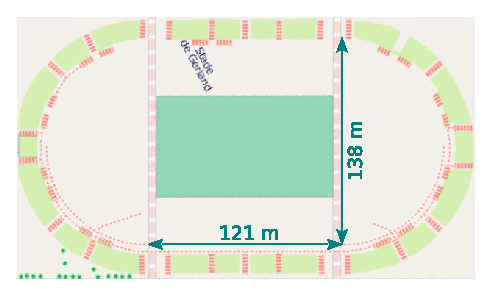
\includegraphics[width=\linewidth]{eeCD09}
\end{center}
\end{exercice}


\begin{exercice}[]
\ImageDroite{Une grande roue d'une fête foraine a un diamètre de 38\,m. Donne une valeur approchée au dixième de...}{\includegraphics[width=.3\linewidth]{roue}}

\hfill {\scriptsize \textit{Source : Wikimedia Commons}}


\begin{colenumerate}{1} 
\item ... la distance parcourue en un tour de grande roue ;
\item ... la distance parcourue en cinq tours de grande roue.
\end{colenumerate} 
\end{exercice}



\serie{Conversions}




\begin{exercice}[]
Recopie et complète.

\begin{colenumerate}{2} 
\item 4\,dam\up{2} = ... m\up{2}
\item 15\,hm\up{2} = ... m\up{2}
\item 5,1\,cm\up{2} = ... mm\up{2}
\item 1 350\,mm\up{2} = ... cm\up{2}
\item 5,2\,km\up{2} = ... m\up{2}
\item 0,7\,m\up{2} = ... dam\up{2}
\item 320\,a = ... m\up{2}
\item 2,5\,ha = ...m\up{2}
\item 15 300\,mm\up{2} = ... cm\up{2} = ... dm\up{2} = ... m\up{2}
\end{colenumerate} 
\end{exercice}

\begin{exercice}[]
Convertis les aires suivantes en m\up{2}.

\begin{colenumerate}{3} 
\item 2\,km\up{2}
\item 37 000\,dm\up{2}
\item 45 300\,mm\up{2}
\item 153,7\,dam\up{2}
\item 28,9\,cm\up{2}
\item 3,008\,hm\up{2}
\item 52\,a
\item 0,05\,ha
\item 200\,ha
\end{colenumerate} 
\end{exercice}


\begin{exercice}[]
Convertis les aires suivantes en cm\up{2}.

\begin{colenumerate}{3} 
\item 15\,mm\up{2}
\item 28\,dm\up{2}
\item 17 300\,mm\up{2}
\item 73,1\,m\up{2}
\item 0,004\,m\up{2}
\item 27,008\,dam\up{2}
\item 0,08\,mm\up{2}
\item 13\,a
\item 0,0105\,a
\end{colenumerate} 
 
\end{exercice}

\begin{exercice}[]
On  donne les superficies suivantes :
\begin{itemize}
    \item Belle-Île-en-mer : 90\,km\up{2}
    \item Île d’Yeu : 2 300\,ha
    \item Île d’Oléron : 175 000 000\,m\up{2}
    \item Île de Jersey : 1 160 000\,dam\up{2}
\end{itemize}

Range ces îles dans l’ordre décroissant de leur superficie.   
\end{exercice}

\begin{exercice}[]
Un jardinier est chargé de la décoration d'un rond-point de 10 mètres de rayon.

\begin{colenumerate}{1} 
\item Il souhaite planter du gazon sur l'intégralité du rond-point. Quelle quantité doit-il prévoir ?
\item Il souhaite planter des fleurs sur le bord extérieur du rond-point, tous les 20\,cm. Combien doit-il prévoir de pots de fleurs ?
\end{colenumerate} 
\end{exercice}



\begin{exercice}[]
Le lac Pavin est un lac français situé dans le Massif Central. Il occupe le cratère presque circulaire d'un ancien volcan. Son diamètre est de 750\,m. 

\begin{colenumerate}{1} 
\item Calcule le périmètre de ce lac. Donne une valeur approchée au mètre près.
\item Calcule l'aire du lac. Donne une valeur approchée à l'hectare près.
\end{colenumerate} 

\end{exercice}



\serie{Disques}



\begin{exercice}[]
Calcule l'aire de chaque disque. Tu donneras la valeur exacte puis une valeur approchée au dixième.

\begin{colenumerate}{2} 
\item Rayon : 4\,cm
\item Rayon : 6\,dm
\item Diamètre : 1,5\,mm 
\item Diamètre : 10,3\,m
\end{colenumerate} 
\end{exercice}

\begin{exercice}[]
Calcule l'aire de chaque disque. Tu donneras la valeur exacte puis une valeur approchée au dixième.

\begin{center}
    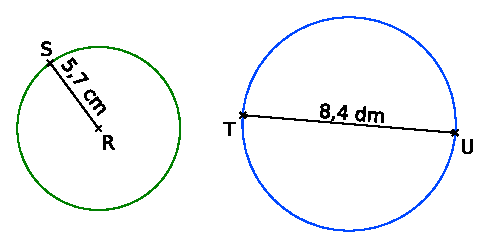
\includegraphics[width=\linewidth]{eeCD11}
\end{center}
\end{exercice}

\begin{exercice}[]
Calcule l'aire de cette figure sachant que sa largeur dans la réalité est de 6,4\,cm.

\begin{center}
    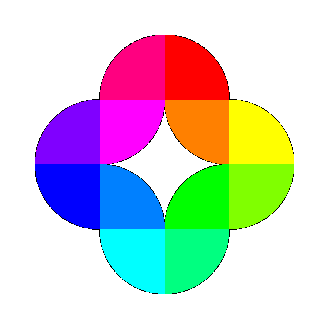
\includegraphics[width=.6\linewidth]{eeCD12}
\end{center}
\end{exercice}


\begin{exercice}[]
Effectue les calculs suivants.

\begin{colenumerate}{1} 
\item L'aire exacte d'un disque de rayon 3\,cm.
\item Une valeur approchée au dixième près de l'aire d'un disque de rayon 35\,mm.
\item L'aire exacte d'un disque de diamètre 8\,cm.
\end{colenumerate} 
\end{exercice}


\begin{exercice}[]
Donne la valeur exacte puis la valeur approchée au centième près de l'aire des disques suivants, où $r$ désigne le rayon du disque et $d$ le diamètre du disque.

\begin{colenumerate}{3} 
\item $r$ = 2\,cm
\item $d$ = 3\,cm
\item $r$ = 4,5\,cm
\item $r$ = 5,6\,cm
\item $d$ = 4,8\,dm
\item $d$ = 0,24\,m
\end{colenumerate} 
 
\end{exercice}

\begin{exercice}[]
Calcule l'aire de chaque figure suivante.
\begin{center}
    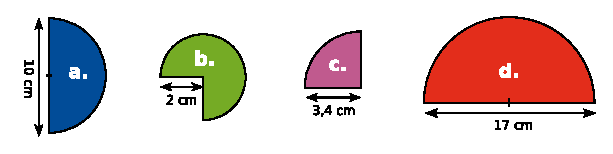
\includegraphics[width=\linewidth]{eeCD13}
\end{center}
\end{exercice}



\begin{exercice}[Portions de disques]

\begin{colenumerate}{1} 
\item Calcule l'aire d'un demi-disque de rayon 5,2\,cm. Donne la valeur exacte puis une valeur approchée au mm\up{2} près.
\item Calcule l'aire d'un quart de disque de rayon 16,4\,cm. Donne la valeur exacte puis une valeur approchée au mm\up{2} près.
\end{colenumerate} 
 
\end{exercice}

\begin{exercice}[]
Recopie et complète le tableau. (On prendra 3,14 comme valeur approchée de $\pi$.)

\renewcommand*\tabularxcolumn[1]{>{\centering\arraybackslash}m{#1}}
\begin{ltableau}{\linewidth}{4}
\hline
Rayon & Diamètre & Périmètre & Aire \\ \hline
5\,cm &   &   &   \\ \hline
 & 2,4\,dm  &   &   \\ \hline
 &   &  6,28\,m &   \\ \hline
 &   &   & 50,24\,cm\up{2}  \\ \hline
\end{ltableau}
\end{exercice}




\begin{exercice}[]
À Mathcity, l'émetteur de \og Radio-Centre \fg a une portée de 10\,km.


\begin{colenumerate}{1} 
\item Calcule la superficie de la zone de réception au km\up{2} près.
\item À partir du mois de septembre prochain, le conseil municipal instaure une taxe de 10 € par km\up{2}. Combien paiera \og radio-centre \fg ?
\item La direction prévoit de changer l'émetteur pour multiplier la portée par 3. La nouvelle taxe sera-t-elle aussi multipliée par 3 ? 
\end{colenumerate} 
\end{exercice}

\begin{exercice}[]
Calcule l'aire et le périmètre de ce stade.
\begin{center}
    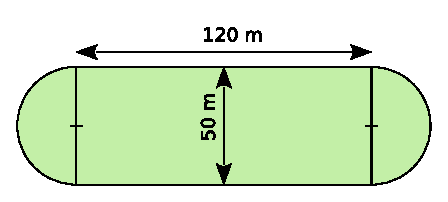
\includegraphics[width=.8\linewidth]{eeCD17}
\end{center}

\end{exercice}

\begin{exercice}[Quadrillage]

\begin{center}
    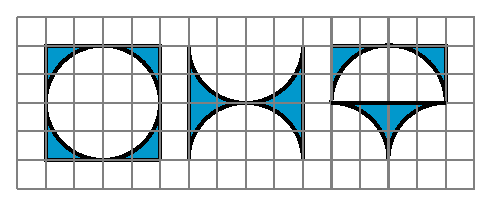
\includegraphics[width=\linewidth]{eeCD18}
\end{center}

Reproduis les figures ci-dessus dans des carrés de 4\,cm de côté puis calcule l'aire de chaque surface coloriée.
\end{exercice}
